
\chapter{Theoretical background} 
\label{ch:THback}

\section{Scalar Diffraction Theory}
\label{sec:ScaDifTh}

A monochromatic wave, at position $P$ and time $t$, can be represented by a scalar field $u(P,t)$ written as :

\begin{equation}
u(P,t) =  A(P) exp\left[-j2\pi\nu t + j\phi(P)\right],
\label{eqt:WvscalarField}
\end{equation}

where $A(P)$ and $\phi(P)$ are the amplitude and phase, respectively, of the wave at position P and $\nu$ is the wave frequency.

The spatial part of eqt. \eqref{eqt:WvscalarField}, also called  phasor  in the literature, $U(P) = A(P)e^{j\phi(P)}$, must verify the Helmotz equation : 

\begin{equation}
(\nabla^2 + k^2)U = 0,
\label{eqt:HelmholtzEqt}
\end{equation}

where $k$ is the wave number given by

\begin{equation}
k = 2\pi n \frac{\nu}{c} = \frac{2\pi}{\lambda},
\label{eqt:wavenumber}
\end{equation}

and $\lambda$ is the wavelength in the dielectric medium.

\begin{figure}
\centering
    \begin{subfigure}{0.4\textwidth}
        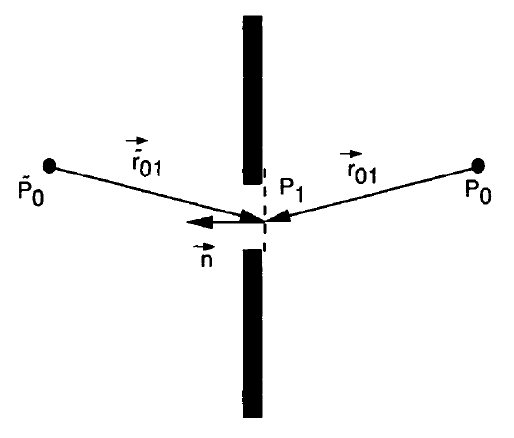
\includegraphics[width=\textwidth]{Figures/Ray_Som_Diff}
        \caption{Rayleigh-Sommerfeld formulation of diffraction by a plane screen.}
        \label{subfig:Ray_Som_Diff}
    \end{subfigure}
    \quad
    \begin{subfigure}{0.5\textwidth}
        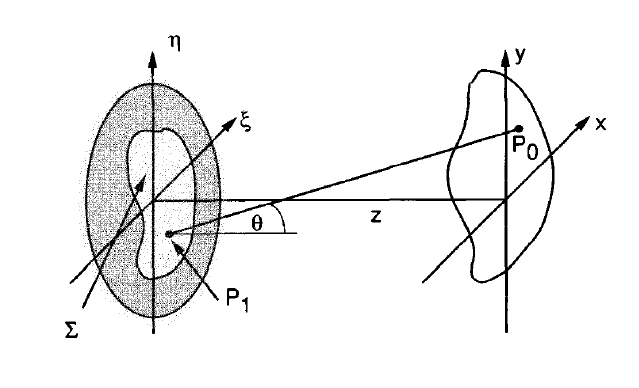
\includegraphics[width=\textwidth]{Figures/Diff_Geom}
        \caption{Diffraction geometry.}
        \label{subfig:Diff_Geom}
    \end{subfigure}
    \decoRule
    \caption{Diffraction Schemas}
    \label{fig:Diff_Schemas}
\end{figure}

Rayleigh and Sommerfeld developed a formalism using the Helmholtz equation and Green's Theorem to compute the induced diffraction by a plane screen. Let's suppose that we have a monochromatic source at $\widetilde{P_0}$ on the left of a plane screen with aperture $\Sigma$, the Rayleigh-Sommerfeld formula allows to compute the complex amplitude at $P_0$ on the right of the plane screen (see Figure \ref{subfig:Ray_Som_Diff}).

\begin{equation}
U(P_0) = \frac{1}{j\lambda} \int\int_{\Sigma} U(P_1)\frac{exp(jkr_{01})}{r_{01}}cos(\mathbf{n},\mathbf{r_{01}})\mathbf{ds}
\label{eqt:Ray_Som_Formula}
\end{equation}

$U(P_1)$ is the complex amplitude on the screen, $cos(\mathbf{n},\mathbf{r_{01}})$ is the cosine of the angle between the aperture plane normal toward the source and the vector $\mathbf{r_{01}} = \mathbf{P_0P_1}$ given by 

\begin{equation}
r_{01} = \sqrt{z^2 + (x-\xi)^2 + (y-\eta)^2}.
\label{eqt:r_01}
\end{equation}

We can rewrite eqt. \eqref{eqt:Ray_Som_Formula} using $cos(\mathbf{n},\mathbf{r_{01}}) = cos(\theta) = \frac{z}{r_{01}}$ and the coordinate systems ($\xi,\eta$) and ($x,y$), see Figure \ref{subfig:Diff_Geom},

\begin{equation}
U(x,y) = \frac{z}{j\lambda} \int\int_{\Sigma} U(\xi,\eta)\frac{exp(jkr_{01})}{r_{01}^2} d\xi d\eta.
\label{eqt:Ray_Som_formula_xy_en}
\end{equation}

\begin{description}
\item[Fresnel Approximation] 
\end{description}